\setcounter{chapter}{18}
\chapter{Claims Triangles}
{\small \textit{Chapter Preview}.  This chapter introduces a classic
actuarial reserving problem that is encountered extensively in
property and casualty as well as health insurance. The data are
presented in a triangular format to emphasize their longitudinal and
censored nature. This chapter explains how such data arise naturally
and introduces regression methods to address the actuarial reserving
problem.}


\section{Introduction}

In many types of insurance, little time elapses between the event of
a claim, notification to an insurance company and payment to
beneficiaries. For example, in life insurance notification and
benefit payments typically occurs within two weeks of an insured's
death. However, for other lines of insurance, times from claim
occurrence to the final payment can be much longer, taking months
and even years. To introduce this situation, this section describes
the evolution of a claim, introduces summary measures used by
insurers and then describes the prevailing deterministic method for
forecasting claims, the chain ladder method.

\subsection{Claims Evolution}\label{S19:ClaimsEvolution}

For example, suppose that you become injured in an automobile
accident covered by insurance. It can take months for the injury to
heal and all of the medical care payments to become known and paid
by the insurance company. Moreover, disputes may arise among you,
other parties to the accident, your insurer and insurer(s) of other
parties, thus lengthening the time until claims are settled and
paid. When claims take a long time to develop, an insurer's claim
obligations may be incurred in one accounting period but not paid
until a later accounting period. In the example of your accident,
the insurer is aware that a claim has occurred and may have even
made some payments in the current accounting period. Future payment
amounts are unknown by the end of the current accounting period but
the insurer wishes to make an accurate forecast of future
obligations to set aside a fair amount of money of future
obligations, known as a \emph{reserve}. The insurer's objective is
to use current claim information to predict the timing and amount of
future claim payments.\index{actuarial \& financial terms and
concepts!reserve}

\marginparjed{The insurer's objective is to use current claim information to predict
the timing and amount of future claim payments.}

To set terminology, it is helpful to follow the timeline of a claim
as it develops. In Figure \ref{F19:TimeLine}, the claim occurs at
time $t_1$ and the insuring company is notified at time $t_3$. There
can be a long gap between occurrence and notification such that a
\emph{valuation date} ($t_2$) may occur within this gap. Here, $t_2$
is the time when the obligations are valued which is typically but
not always at the end of a company financial reporting period. In
this case, the claim is said to be \emph{incurred but not reported}
at this valuation date.\index{actuarial \& financial terms and
concepts!incurred but not reported}\index{actuarial \& financial
terms and concepts!valuation date}

After claim notification, there may one or more loss payments. Not
all of the payments may be made by the next valuation date ($t_4$).
As the claim develops, eventually the company deems its financial
obligations on the claim to be resolved and declares the claim
``closed.'' However, it is possible that new facts arise and the
claim must be re-opened, giving rise to additional loss payments
prior to being closed again.\index{actuarial \& financial terms and
concepts!closed claim}
\begin{figure}[htp]
  \begin{center}
    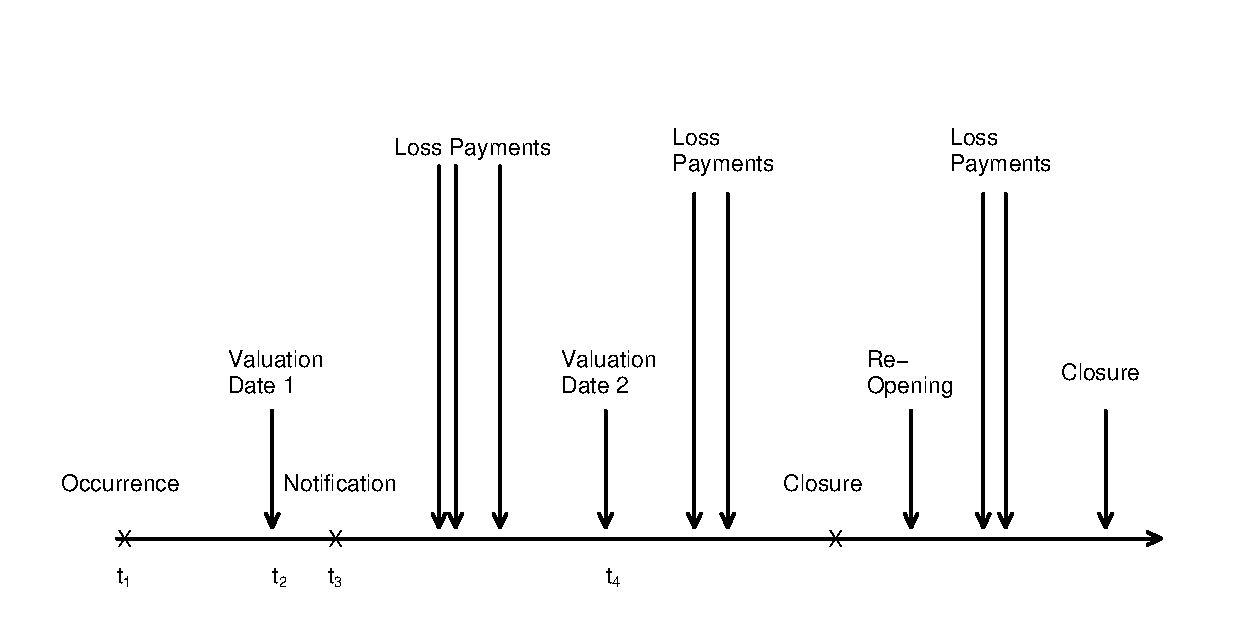
\includegraphics[width=1\textwidth]{Chapter19Triangles/F19TimeLine.eps}
    \caption{\label{F19:TimeLine} \small Timeline of Claim Development.}
  \end{center}
\end{figure}


\subsection{Claims Triangles}\index{claims triangle}

Insurers do not typically model the evolution of each claim and then
sum them (as is done on a policy basis in life insurance). Instead,
portfolios of claims are summarized at each valuation date; it is
these summaries upon which forecasts of outstanding claims are
based.

Specifically, let $i$ represent the year in which a claim has been
incurred and $j$ represent the number of years from incurral to
the time when the payment is made, the ``development'' (or ``delay'') year. Thus,
$y_{ij}$ represents the sum of payment amounts in the $i$th incurral
and $j$th development year. Here, ``year'' refers to the accounting
period - in subsequent examples, you will see that we often use
month, quarter or other fixed period. Table \ref{T19:ClassicRunOff}
shows the information that actuaries typically confront.

\begin{center}  \begin{table}[h]
\caption{\label{T19:ClassicRunOff} Classic Claims Run-Off Triangle}
\begin{tabular}{c|ccccc}
  \hline
  Incurral &    \multicolumn{5}{c}{Development Year ($j$)}     \\
   Year ($i$) & 1& 2& 3&4&5 \\
   \hline
  1  & $y_{11}$  & $y_{12}$ & $y_{13} $&  $y_{14}$ & $y_{15}$  \\
  2  & $y_{21}$  & $y_{22}$ & $y_{23} $&  $y_{24}$ & .      \\
  3  & $y_{31}$  & $y_{32}$ & $y_{33} $&   .       & .      \\
  4  & $y_{41}$  & $y_{42}$ &  .       &.          & .      \\
  5  & $y_{51}$  & .        &  .       &.          & .      \\

  \hline
\end{tabular}
\end{table}  \end{center}

The term ``claims triangle'' is evident from Table
\ref{T19:ClassicRunOff}. We observe data in the upper left-hand
triangle, $y_{ij}, i=1,\ldots, 5, j=1, \ldots,6-i$. The goal is ``to
complete the triangle,'' that is, to forecast values in the lower
right-hand triangle ($y_{ij}, i=2,\ldots, 5, j=7-i, \ldots,5$). For
example, the most recent incurral year is $i=5$ for which we have
only one year of claims experience, $y_{51}$. The other values,
$y_{5j}, j=2, \ldots,5$, are unknown at the valuation date. In some
situations, it is also of interest to forecast claims in development
years six and beyond.

\marginparjed{Claims triangle data are both longitudinal and
censored.}\index{censoring}

Table \ref{T19:ClassicRunOff} underscores the fact that data are
both longitudinal and censored. This is the key point regarding
statistical modeling assumptions. In applications, the observations
can vary significantly depending on the type and purpose. Each
element of the triangle may represent actual payments by the
insurance company, known as ``incremental payments,'' or the
``cumulative'' sum of payments since development. For some lines of
business, estimates of the outstanding payments are available on a
claim-by-claim basis, known as ``case estimates.'' Here, triangle
elements may represent incurred claims in lieu of paid claims. That
is, an incurred claim is the paid amount plus the reserve. Because
case estimates are revised as new information about a claim comes
in, it is not uncommon for incurred payments to be negative.
Further, even paid incremental payments can be negative due to
reinsurance or recovery from other parties of claims amounts. (Many
insurers will write checks to pay claimants quickly upon the
occurrence of an accident and later be reimbursed by another party
responsible for the accident.) Claims triangle data can also be in
the form of the number of claim notifications. This type of data is
particularly useful for estimating ``incurred but not reported''
reserves.\index{actuarial \& financial terms and concepts!case
estimates}\index{actuarial \& financial terms and
concepts!incremental, cumulative payments}

\linejed\index{datasets!Singapore property damage}

\textbf{Example: Singapore Property Damage.}\ecaptionjed{Singapore
Property Damage} Table \ref{T19:SingaporePropertyRunOff} reports
incremental payments from a portfolio of automobile policies for a
Singapore property and casualty (general) insurer. Here, payments
are for third party property damage from comprehensive auto
insurance policies. All payments have been deflated using a
Singaporean consumer price index, so they are in constant dollars.
The data are for policies with coverages from 1997-2001, inclusive.
Table \ref{T19:SingaporePropertyRunOff} also provides the premiums
for these policies (in thousands of Singaporean dollars) to provide
a sense of the insurer's increasing exposure to potential claim
obligations.


\empexjed{SingaporeProperty}

\begin{center}  \begin{table}[h]
\caption{\label{T19:SingaporePropertyRunOff} Singapore Incremental
Payments }
\begin{tabular}{lr|rrrrr}
  \hline
  Incurral &   Premium &\multicolumn{5}{c}{Development Year }     \\
       Year       &  (thousands) &          1 &          2 &          3 &          4 &          5 \\
         \hline
1997 &     32,691 &  1,188,675 &  2,257,909 &    695,237 &    166,812 &     92,129 \\
1998 &     33,425 &  1,235,402 &  3,250,013 &    649,928 &    211,344 &          . \\
1999 &     34,849 &  2,209,850 &  3,718,695 &    818,367 &          . &          . \\
2000 &     37,011 &  2,662,546 &  3,487,034 &          . &          . &          . \\
2001 &     40,152 &  2,457,265 &          . &          . &          . &          . \\
        \hline
\end{tabular}
\end{table}  \end{center}
\linejed



\subsection{Chain Ladder Method}\label{S19:ChainLadder}\index{chain
ladder}

To introduce the basic chain ladder method, we continue to work in
the context of the Singapore property damage example. Table
\ref{T19:SingaporeBasicChainLadder} shows the same payments as Table
\ref{T19:SingaporePropertyRunOff} but in cumulative rather than
incremental form. Let $S_{ij} = y_{i1} + \cdots + y_{ij}$ denote
cumulative claims.

\begin{center}  \begin{table}[h]
\caption{\label{T19:SingaporeBasicChainLadder} Singapore Cumulative Payments with Chain Ladder Estimates}
\scalefont{0.9}
\begin{tabular}{lrrrrrrrr}
 \hline
 \multicolumn{9}{r}{Ultimate}\\
  \multicolumn{9}{r}{Loss }\\
\multicolumn{2}{l}{Incurral }  &\multicolumn{5}{c}{Development Year }  & \multicolumn{2}{r}{Ratio}   \\
Year &  \multicolumn{2}{l}{Premium~~~~~~~1} & \multicolumn{1}{c}{2} &  \multicolumn{1}{c}{3}& \multicolumn{1}{c}{4}&    \multicolumn{1}{c}{5}&    \multicolumn{2}{r}{Reserve~~~ (\%)} \\
\hline
1997 &     32,691 &  1,188,675 &  3,446,584 &  4,141,821 &  4,308,633 &  4,400,762 &            &       13.5 \\
\cline{7-7}1998 &     33,425 &  1,235,402 &  4,485,415 &  5,135,343 &  5,346,687 & {\bf 5,461,012} &    114,325 &       16.3 \\
\cline{6-6}1999 &     34,849 &  2,209,850 &  5,928,544 &  6,746,912 & \multicolumn{1}{r}{\bf 7,021,930} &  {\bf 7,172,075} &    425,163 &       20.6 \\
\cline{5-5}2000 &     37,011 &  2,662,546 &  6,149,580 & {\bf 7,109,486} & {\bf 7,399,283} & {\bf 7,557,497} &  1,407,917 &       20.4 \\
\cline{4-4}2001 &     40,152 &  2,457,265 &{\bf 6,738,898} & {\bf 7,790,792} & {\bf 8,108,361} & {\bf 8,281,737} &  5,824,471 &       20.6 \\
\hline
\multicolumn{3}{l}{Total Reserve}        &       &    &       &       & 7,771,877 \\
\multicolumn{3}{l}{Chain Ladder Factors} &       2.742 &      1.156 &      1.041 &      1.021 &  \\
 \hline
\end{tabular}\scalefont{1.1111}
\end{table}  \end{center}

The chain ladder factor for the $j$th development year is calculated
by taking the ratio of the sum of claims over all incurral years for
the $j$th development year divided by the sum of the same incurral
year payments for the  $j-1^{st}$ development year. Using notation,
we have
\begin{equation*}
CL_j = \frac {\sum_{i=1}^{6-j} S_{ij}}{\sum_{i=1}^{6-j} S_{i,j-1}}.
\end{equation*}
For example, $CL_5 = 4,400,762/4,308,633 = 1.021 $ and $CL_4 =
(5,346,687+4,308,633)/(5,135,343+4,141,821)= 1.041 $.

Bold numbers are forecasts calculated recursively using the chain
ladder factors and $\widehat{S}_{i,j} = CL_{j} \times
\widehat{S}_{i,j-1}.$ The recursion starts when the value of the
cumulative payment is known so that $\widehat{S}_{ij}=S_{ij}$. For
example, for incurral year 2, $\widehat{S}_{25} = CL_5 \times S_{24}
= (1.021)(5,346,687)=5,461,012$. For incurral year 3,
$\widehat{S}_{34} = CL_4 \times S_{33} =
(1.041)(6,746,912)=7,021,930$ and $\widehat{S}_{35} = CL_5 \times
\widehat{S}_{34} = (1.021)(7,021,930)=7,172,075$. Alternatively, one
can go directly to the last development year and use
$\widehat{S}_{35} = CL_5 \times \widehat{S}_{34} = CL_5 \times CL_4
\times S_{33} = (1.041)(1.021)(6,746,912)=7,172,075.$

In Table \ref{T19:SingaporeBasicChainLadder}, the reserve is the
ultimate forecast amount minus the most recent cumulative paid
claim. The ultimate loss ratio is the ratio of the forecast of
cumulative claims in the last development year (5) to premiums paid
(expressed as a percentage, recall that premiums are in thousands).

\section{Regression Using Functions of Time as Explanatory
Variables}\label{S19:RegressionFunction}

The chain ladder method is an important tool that actuaries use
extensively when forecasting claims. It is typically presented as
deterministic, as in Section \ref{S19:ChainLadder}. Alternative
stochastic models for claim forecasting have two primary advantages.
\begin{itemize}
\item By explicitly modeling the distribution of claims, estimates
for the uncertainty of the reserve forecasts can be made.
\item There are
many variations of chain ladder techniques available because they
are applied in many different situations. As we have seen in Chapter
5, stochastic methods feature a disciplined way of model selection
that can help determine the most appropriate model for a given set
of data. \end{itemize}

As we will see, one need not make a choice between using the chain
ladder method and a stochastic model. The Section \ref{S19:Poisson}
overdisperse Poisson model and the Section 19.3 Mack model both
yield point forecasts that are equal to chain ladder forecasts.

\subsection{Lognormal Model}

Our starting point is the lognormal model for incremental claims.
That is, we consider a two factor model of the form

\begin{equation}\label{E19:LogNormal}
\ln y_{ij} = \mu + \alpha_i + \tau_j + \varepsilon_{ij},
\end{equation}
where $\{ \alpha_i \}$ are parameters for the incurral year factor
and $\{ \tau_j \}$ are parameters for the development year factor. A
regression model with two factors was introduced in Section 4.4.
Recall that we require constraints on the factor parameters for
estimability such as $\sum_i \alpha_i = 0$ and $\sum_j \tau_j= 0$.
Assuming normality of $\{\varepsilon_{ij} \}$ gives rise to the
lognormal specification for the incremental claims $y_{ij}$.

\linejed\index{datasets!Singapore third party injury}

\textbf{Example: Singapore Third Party
Injury.}\ecaptionjed{Singapore Injury} Table
\ref{T19:SingaporeInjuryRunOff} reports payments from a portfolio of
automobile policies for a Singapore property and casualty (general)
insurer. Payments, deflated for inflation, are for third party
injury from comprehensive insurance policies. The data are for
policies with coverages from 1993-2001, inclusive.

\empexjed{SingaporeInjury}

In automobile insurance, it typically takes longer to settle and pay
injury compared to property damage claims. Thus, the number of
development years, ``the run-off,'' is longer  in Table
\ref{T19:SingaporeInjuryRunOff} than Table
\ref{T19:SingaporePropertyRunOff}. Table
\ref{T19:SingaporeInjuryRunOff} also shows a lack of stability of
injury payments that Figure \ref{F19:Payments} helps us visualize.
The left-hand panel shows trend lines by development for each
incurral year. The right-hand panel presents box plots of
logarithmic payments for each development year. This display shows
that payments tend to rise for the first two development periods
($j=1,2$), reach a peak at the third period ($j=3$) and decline
thereafter.\index{actuarial \& financial terms and concepts!run-off}



\begin{center}  \begin{table}[h]
\caption{\label{T19:SingaporeInjuryRunOff} Singapore Incremental
Injury Payments, 1993-2001} \scalefont{0.9}
\begin{tabular}{c|rrrrrrrrr}
  \hline
Incurral&\multicolumn{9}{c}{Development Year }     \\
Year & 1 & 2 &3 &4 & 5 & 6 & 7 & 8 & 9 \\
         \hline
1993 &    14,695 &    205,515 &    118,686 &    416,286 &     93,544 &    185,043 &     37,750 &     0 &14,086 \\
1994 &   153,615 &    467,722 &    645,513 &    421,896 &    146,576 &     96,470 &     27,765 &38,017 &   . \\
1995 &    24,741 &    547,862 &    754,475 &    417,573 &    156,596 &     55,155 &     36,984 &  . &  . \\
1996 &    68,630 &    188,627 &    492,306 &    179,249 &     34,062 &    443,436 &          . &  . &   . \\
1997 &    29,177 &    364,672 &    437,507 &    385,571 &    529,319 &          . &          . & . &  . \\
1998 &    40,430 &    241,809 &    678,541 &    528,026 &          . &          . &          . & . &  . \\
1999 &    45,125 &    372,935 &    704,168 &          . &          . &          . &          . & . &  . \\
2000 &    21,695 &    158,005 &          . &          . &          . &          . &          . & . & . \\
2001 &     6,626 &          . &          . &          . &          . &          . &          . &  . & . \\
        \hline
\end{tabular}
\scalefont{1.1111}
\end{table}  \end{center}


\begin{figure}[htp]
  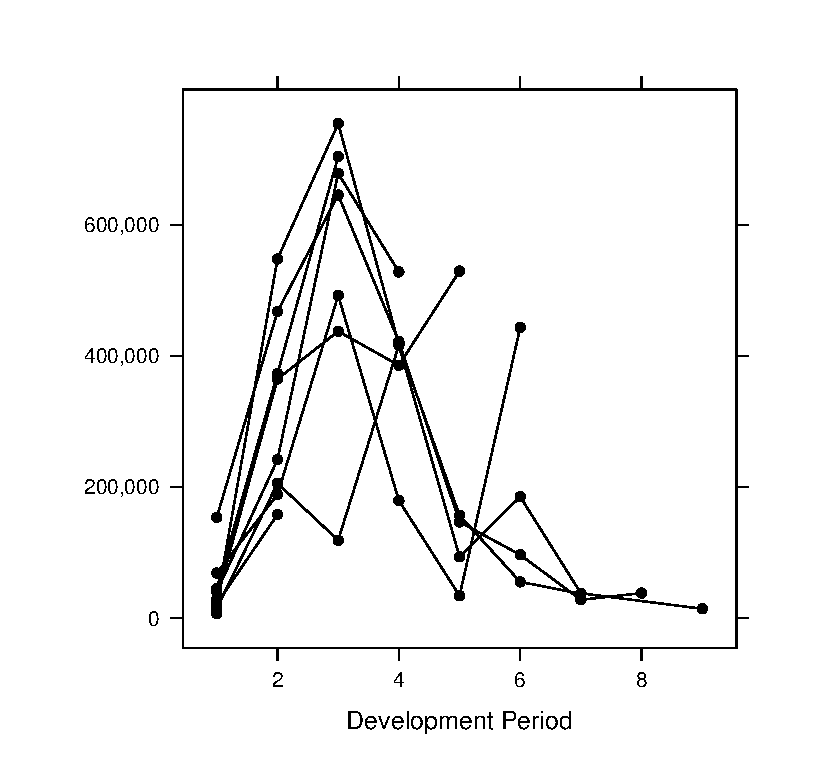
\includegraphics[width=0.48\textwidth]{Chapter19Triangles/F19PaymentMTimeSeries.eps}
  \hfill
    $~~~~~$
   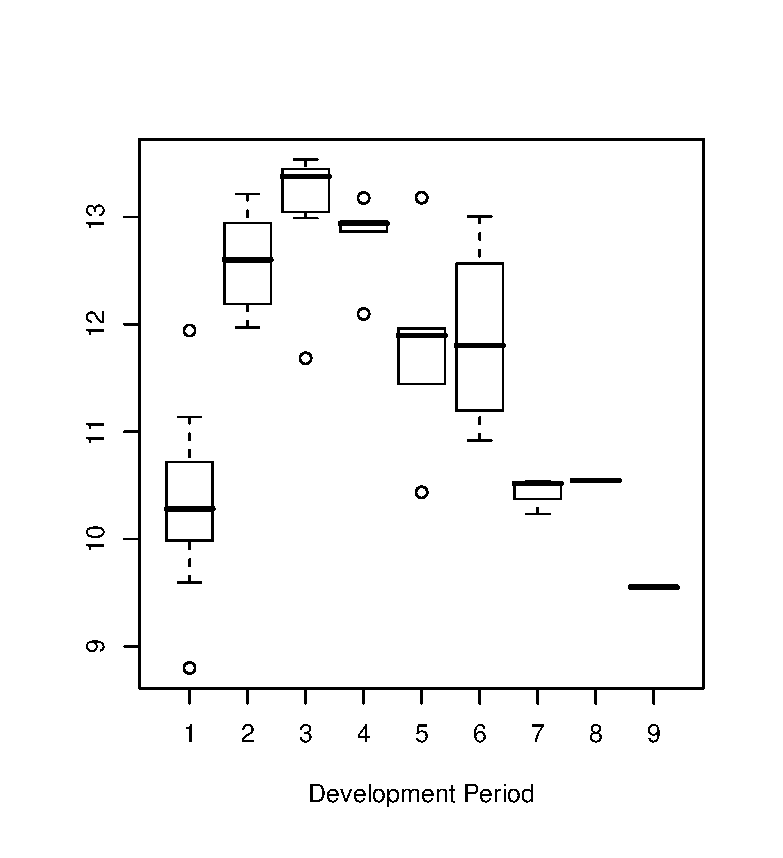
\includegraphics[width=0.45\textwidth]{Chapter19Triangles/F19PaymentBoxPlotLog.eps}
  \caption{\label{F19:Payments} \small {Singapore Incremental
Injury Payments. The left-hand panel shows payments by development
year with each line connecting payments from the same incurral year.
The right-hand panel shows the distribution of logarithmic payments
for each development year.}}
\end{figure}
\newpage

The lognormal model based on equation (\ref{E19:LogNormal}) was fit
to these data. Not surprisingly, both factors incurral and
development year were statistically significant. The coefficient of
determination from the fit is $R^2 = 73.3 \%$. A $qq$ plot (not
presented here) showed reasonable agreement with the assumption of
normality. Fitted values from the model, after exponentiation to
convert back to dollars, appear in Figure
\ref{F19:PaymentFittedValues}. This figure seems to capture the
payment patterns that appear in the left-hand panel of Figure
\ref{F19:Payments}. Note that the fitted values for the unobserved
portion of the triangle are forecasts.



\begin{figure}[htp]
    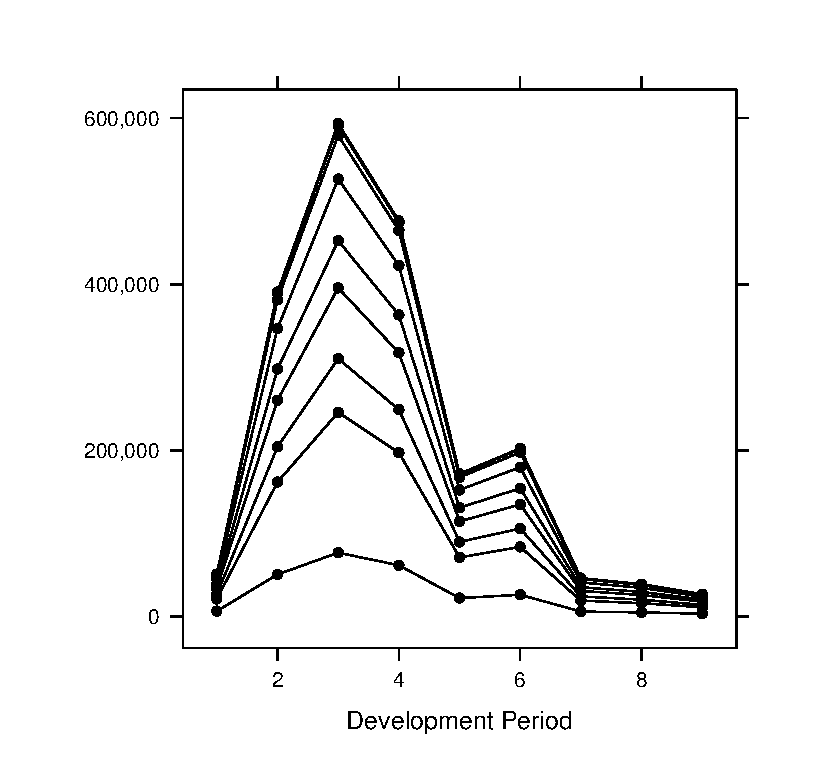
\includegraphics[width=0.6\textwidth]{Chapter19Triangles/F19PaymentFittedValues.eps}
  \caption{\label{F19:PaymentFittedValues} Fitted Values for the Singapore Incremental
Injury Payments. These estimates are based on the two factor
lognormal model.}
\end{figure}

\linejed

\subsection{Hoerl Curve}

The systematic component of equation (\ref{E19:LogNormal}) can be
easily modified. One possibility is the so-called ``Hoerl curve,''
leading to the model equation

\begin{equation}\label{E19:Hoerl}
\ln y_{ij} = \mu + \alpha_i + \beta_i \ln (j) + \gamma_i \times j +
\varepsilon_{ij} .
\end{equation}
An advantage of treating development time $j$ as a continuous
covariate is that extrapolation is possible beyond the range of
development times observed. As a variation, England and Verrall
(2002) suggest allowing the first few development years to have
their own levels and imposing the same run-off pattern for all
incurral years ($\beta_i = \beta$, $\gamma_i = \gamma$).

\linejed

\textbf{Example: Singapore Third Party Injury - Continued.} The
basic model from equation (\ref{E19:Hoerl}) fit well, the
coefficient of determination is $R^2 = 87.8 \%$. We also examined a
simpler model based on the equation
\begin{equation}\label{E19:ReducedHoerl}
\ln y_{ij} = \mu + \alpha_i +  \beta \ln (j) + \gamma \times j +
\varepsilon_{ij} .
\end{equation}
This simpler model did not fit the data as well as the more complete
Hoerl model from equation (\ref{E19:Hoerl}), having $R^2 = 78.6\%$.
However, a partial $F$ test established that the additional
parameters were not statistically significant and so the simpler
model in equation (\ref{E19:ReducedHoerl}) is preferred.

Based on the simpler model, fitted values are displayed in Figure
\ref{F19:HoerlFittedValues}. This figure displays the geometrically
declining fitted values beginning in the fourth development period.



\begin{figure}[htp]
    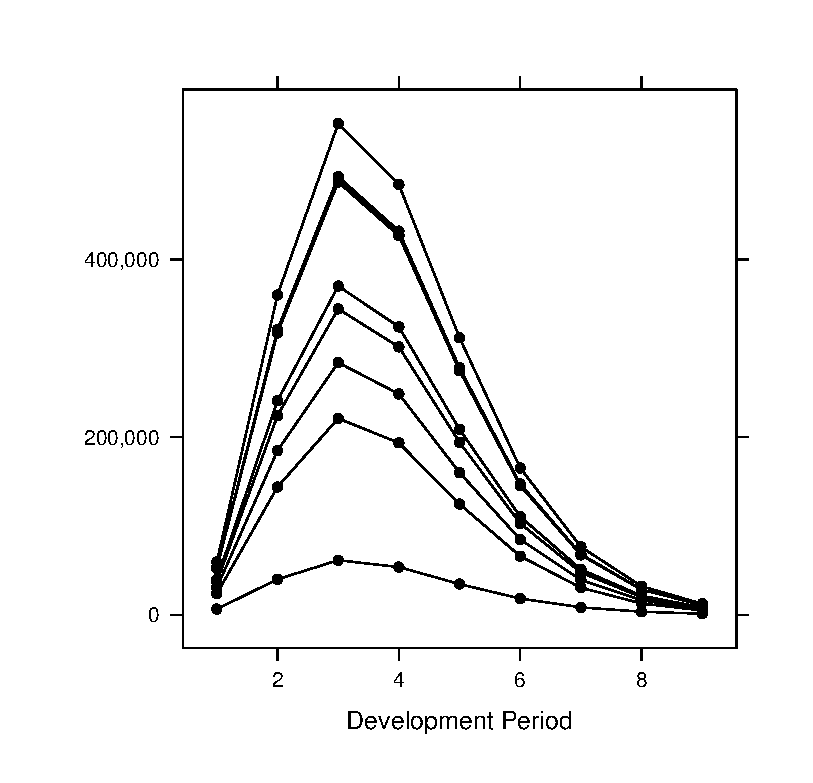
\includegraphics[width=0.6\textwidth]{Chapter19Triangles/F19HoerlFittedValues.eps}
  \caption{\label{F19:HoerlFittedValues} Fitted Values from the Reduced Hoerl Model in Equation (\ref{E19:ReducedHoerl}).}
\end{figure}

\linejed

\subsection{Poisson Models}\label{S19:Poisson}\index{regression
model!count!overdisperse Poisson}\index{distributions!Poisson}

A drawback of the lognormal model is that the predictions produced
by it do not replicate the traditional chain-ladder estimates. This
section introduces the overdisperse Poisson model that does have
this desirable feature.

To begin, from equation (\ref{E19:LogNormal}), we may write
\begin{equation*}
\mathrm{E}~ y_{ij} = \exp(\eta_{i,j}) \mathrm{E}~ e^{\varepsilon}
\end{equation*}
where the systematic component is $\eta_{i,j} = \mu + \alpha_i +
\tau_j$. This is a model with a logarithmic link function (that is,
$\ln \mathrm{E}~y = \eta$). Instead of using the lognormal
distribution for $y$, this section assumes that $y$ follows an
overdisperse Poisson with variance function
\begin{equation*}
\mathrm{Var}~ y_{ij} = \phi \exp(\eta_{i,j}).
\end{equation*}
Note that we have absorbed the scalar $\mathrm{E}~ e^{\varepsilon}$
into the overdispersion parameter $\phi$.

We introduced overdisperse Poisson models in Section 12.3. Thus,
this model can be estimated with standard statistical software and,
as with the lognormal model, forecasts readily produced. It can be
shown that the forecasts produced by the overdisperse Poisson are
equivalent to the deterministic chain ladder forecasts. See, for
example Taylor (2000) or W\"{u}thrich and Merz (2008) for a proof.
Not only does this give us a mechanism to quantify the uncertainty
associated with chain ladder forecasts, we can also use standard
statistical software to compute these estimates.

\linejed

\textbf{Example: Singapore Third Party Injury - Continued.} The
overdisperse Poisson model was fit to the Singapore injury payments
data. Standard statistical software was use to compute parameter
estimates, using techniques described in Section 12.3. Figure
\ref{F19:PoissonCumForecasts} summarizes the forecasts from these
models. This figure shows cumulative, not incremental, payments,
marked with opaque plotting symbols in the figure. Forecasts of
incremental payments were produced and then summed to get the
cumulative payment forecasts in Figure
\ref{F19:PoissonCumForecasts}; these are marked with the open
plotting symbols. The reader is invited to check that these
forecasts are identical to those produced by the deterministic chain
ladder method up to the eight development year. Here, the value of
zero for the first incurral year causes small differences between
the Poisson model and chain ladder forecasts.

\begin{figure}[htp]
    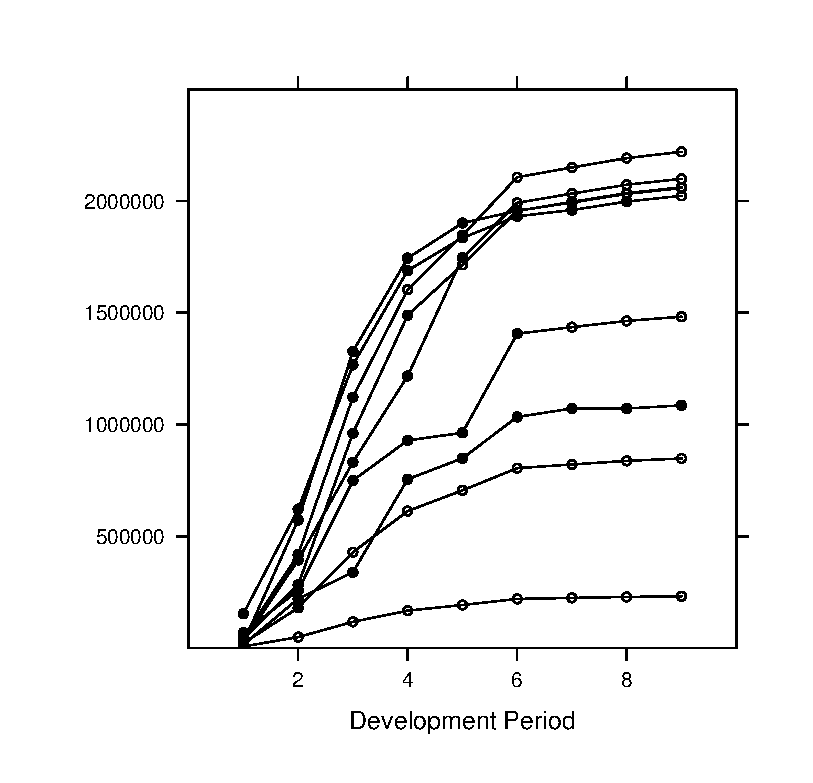
\includegraphics[width=0.6\textwidth]{Chapter19Triangles/F19PoissonCumForecasts.eps}
  \caption{\label{F19:PoissonCumForecasts} Actual and Forecast Values for the Singapore
  Cumulative Injury Payments. Actual values are denoted with an
  opaque plotting symbol. Chain ladder forecasts, from an
  overdisperse Poisson model, are denoted with an open plotting
  symbol.}
\end{figure}

\linejed


\section{Using Past Developments}

As with autoregressive models, one can use prior history to forecast
payments. What is prior history? In the claim triangle set-up in
Table \ref{T19:ClassicRunOff}, there are \emph{two} dimensions of
time: incurral year and development year. Most models focus on using
prior development (``$j$'') for forecasting. By focusing on prior
development experience, we allow ourselves the flexibility to our
model cumulative ($S_{ij}$) or incremental ($y_{ij}$) payments. As
we learned in our Chapters 7 and 8 study of time series, it is
useful to be able to model both a series ($S_{ij}$) and its changes
($y_{ij} = S_{ij}-S_{i,j-1}$).


\subsection{Mack Model}

The model put forward by Mack (1993) specifies the first two
conditional moments of cumulative payments and uses generalized
least squares to fit the model. Under this stochastic specification,
traditional chain ladder forecasts are produced.

Specifically, we assume

\begin{equation}\label{E19:MackMoment1}
\mathrm{E} \left( S_{i,j} | S_{i,j-1} \right) = \nu_j  S_{i,j-1}
\end{equation}
and
\begin{equation}\label{E19:MackMoment2}
\mathrm{Var} \left( S_{i,j} | S_{i,j-1} \right) = \sigma^2_j ,
S_{i,j-1}
\end{equation}
where $\nu_j$ and $\sigma^2_j$ are model parameters.

The mean parameters, $\nu_j$, are determined through generalized
least squares by minimizing the quantity
\begin{equation*}
Q = \sum_{j=2}^n \sum_{i=1}^{n+1-i}
 \frac{(S_{ij} - \nu_j S_{i,j-1})^2}{\sigma_j^2 S_{i,j-1}} .
 \end{equation*}
Taking derivatives with respect to the parameters $\nu_j$ and
setting them equal to zero yields
\begin{equation*}
\frac{\partial}{\partial \nu_j}Q = \sum_{i=1}^{n+1-i}
     \frac{(-2) (S_{ij} - \nu_j S_{i,j-1})}{\sigma_j^2 S_{i,j-1}} =0.
\end{equation*}
The solution of this equation yields
\begin{equation*}
\hat{\nu_j}= \frac{\sum_{i=1}^{n+1-i} S_{ij}} {\sum_{i=1}^{n+1-i}
S_{i,j-1}},
 \end{equation*}
the chain-ladder factor. Here, the carat, or ``hat,'' on $\nu_j$
indicates that $\hat{\nu_j}$ is an estimator determined by the data.

With these parameter estimates, one can use equation
(\ref{E19:MackMoment1}) to produce fitted values that equal
chain-ladder estimates. Moreover, one can estimate the scale
parameters $\sigma^2_j$ and then use equation
(\ref{E19:MackMoment2}) to quantify the uncertainty of the
estimates. See England and Verrall (2002) or W\"{u}thrich and Merz
(2008) for details on the scale parameter estimation.

The strength and limitation of this model is that it only employs
assumptions about the first two conditional moments. It is a
strength in the sense that we need not worry about whether the
underlying distribution is close to lognormal or Poisson. Thus, it
is sometimes referred to as a ``nonparametric'' model. It is a
limitation in the sense that measures of uncertainty in equation
(\ref{E19:MackMoment2}) are related to the second moment that uses a
squared error loss function. For insurance claims, data are
typically skewed so that the variance is not a good scale measure.
Moreover, in loss reserving, we want to know if reserves are too
high or too low; using a measure of uncertainty that only reports
absolute deviations does not provide the actuary with the type of
information needed.


\subsection{Distributional Models}

Models supplementing the moment assumptions in equations
(\ref{E19:MackMoment1}) and (\ref{E19:MackMoment2}) with
distributional assumptions on payments have been proposed in the
literature.\index{regression model!count!negative binomial GLM}

For example, Verrall proposed using the negative binomial as a
distribution for $\{y_{ij}\}$ with conditional moments

\begin{equation*}
\mathrm{E} \left( y_{i,j} | S_{i,j-1} \right) = (\nu_j-1) S_{i,j-1}
\end{equation*}
and
\begin{equation*}
\mathrm{Var} \left( y_{i,j} | S_{i,j-1} \right) = \phi \nu_j (\nu_j
-1) S_{i,j-1}
\end{equation*}
where $\phi$ and $\nu_j$ are model parameters. Note that the
conditional mean assumption is the same as equation
(\ref{E19:MackMoment1}) because of the relation $\mathrm{E} \left(
S_{i,j} | S_{i,j-1} \right) = S_{i,j-1} + \mathrm{E} \left( y_{i,j}
| S_{i,j-1} \right)$. Similarly, we can express the variance of
cumulative payments as $\mathrm{Var} \left( S_{i,j} | S_{i,j-1}
\right) = \mathrm{Var} \left( y_{i,j} | S_{i,j-1} \right)$. Thus,
the conditional variance assumption is as in equation
(\ref{E19:MackMoment2}) with parameters $ \sigma^2_j=\phi \nu_j
(\nu_j -1)$. This model can be easily implemented using generalized
linear model software by specifying the negative binomial model with
logarithmic link function
\begin{equation*}
\ln \mu_{ij} = \ln \lambda_j + \ln S_{i,j-1},
\end{equation*}
where $\mu_{ij} = \mathrm{E} \left( y_{i,j} | S_{i,j-1} \right)$.
See England and Verrall (2002, Section 7.3) for further discussion.

Another distributional model, suggested by England and Verrall
(2002, Section 2.5) is to use the moments in equations
(\ref{E19:MackMoment1}) and (\ref{E19:MackMoment2}) but specify a
normal distribution for payments $\{y_{ij} \}$. This can be useful
as an approximation to the negative binomial model, particularly in
the case when estimates of $\nu_j$ are less than one indicating that
the conditional variance is misspecified.

As emphasized at the beginning of Section
\ref{S19:RegressionFunction}, the important strength of the
distributional models are that (1) they allow analysts to quantify
the uncertainty of the forecasts and (2) provide disciplined
mechanisms for model selection.


\section{Further Reading and References}

Two book-long introductions to claim triangles are Taylor (2000) and
W\"{u}thrich and Merz (2008). Practicing actuaries will find the
review article by England and Verrall (2002) to be helpful.

When there is instability in the run-off patterns in the early
years, a method developed by Bornheuetter and Ferguson (1972) can be
useful in that it allows the actuary to incorporate an external
assessment of ultimate paid claims. As with the chain-ladder, this
technique can be expressed in terms of stochastic modeling via
Bayesian modeling. See, for example, the discussion by England and
Verrall (2002), W\"{u}thrich and Merz (2008) and de Alba (2006).

An emerging problem is developing reserves when one triangle is
correlated with another. Such correlation might be expected among
lines of insurance business. Braun (2004) provides an introduction
to this topic.

Another emerging area is developing reserve based on individual
claims run-off patterns, such as described in Section
\ref{S19:ClaimsEvolution}. Antonio et al. (2006) provides an
introduction to this topic, where they use mixed linear models to
develop reserves for claims that have been reported but not yet
settled. See also Section 14.5 on recurrent event theory.

\bigskip

\textbf{Chapter References}

\begin{multicols}{2}

\scalefont{0.9}

de Alba, Enrique (2006). Claims reserving when there are negative
values in the runoff triangle: Bayesian analysis using the
three-parameter log-normal distribution. \emph{North American
Actuarial Journal} 10 (3), 45-59.

Antonio, Katrien, Jan Beirlant, Tom Hoedemakers and Robert Verlaak
(2006). Lognormal mixed models for reported claim reserves.
\emph{North American Actuarial Journal} 10 (1), 30-48.

Bornheuetter, Ronald L. and Ronald E. Ferguson (1972). The actuary
and IBNR. \emph{Proceedings of the Casualty Actuarial Society} 59,
181-195.

Braun, Christian (2004). The prediction error of the chain ladder
method applied to correlated run-off triangles. \textit{Astin
Bulletin} 34 (2), 399-423.

England, Peter D. and Richard J. Verrall (2002). Stochastic claims
reserving in general insurance. \emph{British Actuarial Journal} 8,
443-544.

Gamage, Jinadasa, Jed Linfield, Krzysztof Ostaszewski and Steven
Siegel (2007). Statistical methods for health actuaries - IBNR
estimates: An introduction. Society of Actuaries working paper,
Society of Actuaries, Schaumburg IL.

Mack, Thomas (1993). Distribution-free calculation of the standard
error of chain-ladder reserve estimates. \emph{ASTIN Bulletin} 23
(2), 213-225.

Mack, Thomas (1994). Measuring the variability of chain-ladder
reserve estimates. \emph{Casualty Actuarial Society}, Spring Forum.

Taylor, Greg (2000). \emph{Loss Reserving: An Actuarial
Perspective}. Kluwer Academic Publishers, Boston.

Wacek, Michael G. (2007). The path of the ultimate loss ratio
estimate. \textit{Variance} 1(2), 173-192.

W\"{u}thrich, Mario V. and Michael Merz (2008). \emph{Stochastic
Claims Reserving Methods in Insurance.} Wiley, New York.

\scalefont{1.1111}

\end{multicols}


\bigskip

\section{Exercises}

\begin{exercises}

\scalefont{0.90}


\item \label{Ex19:Ex1} The data in Table \ref{T19:EnglandVerrall} originate from
the 1991 edition of the ``Historical Loss Development Study''
published by the Reinsurance Association of American (page 91).
These data have been widely used to illustrate triangle methods,
beginning with Mack (1994) and later by England and Verrall (2002).
These data are from automatic facultative reinsurance business in
general liability (excluding asbestos and environmental) coverages.
(Under a facultative basis, each risk is underwritten by the
reinsurer on its own merits.) Table \ref{T19:EnglandVerrall} reports
incremental incurred losses from 1981-1990, in thousands of US
dollars.

\empexjed{ReinsGenLiab}\index{datasets!general liability
reinsurance}


a. Begin by calculating the deterministic chain ladder factors. Note
the element in the second origin and seventh development year is
negative. You may wish to first convert the incremental to
cumulative payments. Use these factors to ``complete the triangle.''

b. Use your work in part (a) to calculate the reserve estimate.

c. Remove the observation in the second origin and seventh
development year. Fit a lognormal model to the remaining data.
Comment on the statistical significance of each factor and the
goodness of fit.

d. Fit the Hoerl model to the data in part (c). Produce a graph of
fitted values.

e. Fit the overdisperse Poisson model to the data in part (c). Check
the proximity of these fitted values to the chain ladder values
produced in part (a).


\begin{table}[h]
\scalefont{0.9} \caption{\label{T19:EnglandVerrall} Loss Development
Study (1991) Facultative Reinsurance}
\begin{tabular}{crrrrrrrrrr}
\hline
      Year &          1 &          2 &          3 &          4 &          5 &          6 &          7 &          8 &          9 &         10 \\
\hline         1 &      5,012 &      3,257 &      2,638 &        898 &      1,734 &      2,642 &      1,828 &        599 &         54 &        172 \\
         2 &        106 &      4,179 &      1,111 &      5,270 &      3,116 &      1,817 &       -103 &        673 &        535 &            \\
         3 &      3,410 &      5,582 &      4,881 &      2,268 &      2,594 &      3,479 &        649 &        603 &            &            \\
         4 &      5,655 &      5,900 &      4,211 &      5,500 &      2,159 &      2,658 &        984 &            &            &            \\
         5 &      1,092 &      8,473 &      6,271 &      6,333 &      3,786 &        225 &            &            &            &            \\
         6 &      1,513 &      4,932 &      5,257 &      1,233 &      2,917 &            &            &            &            &            \\
         7 &        557 &      3,463 &      6,926 &      1,368 &            &            &            &            &            &            \\
         8 &      1,351 &      5,596 &      6,165 &            &            &            &            &            &            &            \\
         9 &      3,133 &      2,262 &            &            &            &            &            &            &            &            \\
        10 &      2,063 &            &            &            &            &            &            &            &            &            \\
\hline
\end{tabular}
\scalefont{1.1111}
\end{table}

\newpage


\item The data in Table \ref{T19:BraunGenLiab} is an excerpt from Braun
(2004) that is based on the 2001 edition ``Historical Loss
Development Study'' published by the Reinsurance Association of
American. The larger data (available in the file ``ReinsGL2004'')
contains data for years 1987-2000, inclusive.

Repeat parts (a)-(e) of Exercise \ref{Ex19:Ex1} for these data.

\empexjed{ReinsGL2004}\index{datasets!general liability reinsurance}
\begin{table}[h]
 \caption{\label{T19:BraunGenLiab} Reinsurance General Liability}
\begin{center}
\scalefont{0.9}
\begin{tabular}{lrrrrrr}
\hline
      Year &          1 &          2 &          3 &          4 &          5 &          6           \\
\hline
      1995 &     97,518 &    343,218 &    575,441 &    769,017 &    934,103 &   1,019,303           \\
      1996 &    173,686 &    459,416 &    722,336 &    955,335 &   1,141,750 &                      \\
      1997 &    139,821 &    436,958 &    809,926 &   1,174,196 &            &                      \\
      1998 &    154,965 &    528,080 &   1,032,684 &            &            &                      \\
      1999 &    196,124 &    772,971 &            &            &            &                      \\
      2000 &    204,325 &            &            &            &            &                      \\
\hline
\end{tabular}
\scalefont{1.1111}
\end{center}
\end{table}




\item The data in Table \ref{T19:Wacek} are from Wacek
(2007). The data represent industry aggregates for private passenger
auto liability/medical coverages from year 2004, in millions of
dollars. They are based on insurance company annual statements,
specifically, Schedule P, Part 3B. The elements of the triangle
represent cumulative net payments, including defense and cost
containment expenses.

\empexjed{AutoIndustry}\index{datasets!auto industry claim triangle}

Repeat parts (a)-(e) of Exercise \ref{Ex19:Ex1} for these data.



\begin{center}  \begin{table}[h]
\scalefont{0.9} \caption{\label{T19:Wacek} 2004 US Insurance
Industry Aggregates for Private Passenger Auto Liability and Medical
}
\begin{tabular}{rrrrrrrrrrr}
\hline
      Year &          1 &          2 &          3 &          4 &          5 &          6 &          7 &          8 &          9 &         10 \\
\hline
      1995 &     17,674 &     32,062 &     38,619 &     42,035 &     43,829 &     44,723 &     45,162 &     45,375 &     45,483 &     45,540 \\
      1996 &     18,315 &     32,791 &     39,271 &     42,933 &     44,950 &     45,917 &     46,392 &     46,600 &     46,753 &            \\
      1997 &     18,606 &     32,942 &     39,634 &     43,411 &     45,428 &     46,357 &     46,681 &     46,921 &            &            \\
      1998 &     18,816 &     33,667 &     40,575 &     44,446 &     46,476 &     47,350 &     47,809 &            &            &            \\
      1999 &     20,649 &     36,515 &     43,724 &     47,684 &     49,753 &     50,716 &            &            &            &            \\
      2000 &     22,327 &     39,312 &     46,848 &     51,065 &     53,242 &            &            &            &            &            \\
      2001 &     23,141 &     40,527 &     48,284 &     52,661 &            &            &            &            &            &            \\
      2002 &     24,301 &     42,168 &     50,356 &            &            &            &            &            &            &            \\
      2003 &     24,210 &     41,640 &            &            &            &            &            &            &            &            \\
      2004 &     24,468 &            &            &            &            &            &            &            &            &            \\
\hline
\end{tabular}
\scalefont{1.1111}
\end{table}
\end{center}



\item The data in Table 19.8 are from Gamage et al.
(2007). These data for 36 months of medical care payments, from
January 2001 through December 2003, inclusive. These are payments
for medical care coverage with no deductible nor coinsurance. There
were relatively low co-payments, such as \$10 per office visit. The
payments exclude prescription drugs that typically have a shorter
payment pattern compared with other medical claims.

\empexjed{MedicalCare}\index{datasets!medical care payment triangle}

Repeat parts (a)-(e) of Exercise \ref{Ex19:Ex1} for these data.

\newpage
\begin{sidewaystable}\label{T19:SoAHealth}
\begin{center}
\scalefont{0.7}
\begin{tabular}{lrcrrrrrrrrrrrrr}
\multicolumn{16}{c}{\large Table 19.8.  Monthly Medical Care Payments, 2001-2003} \\
 \hline
      Date &    Members &      Month &          1 &          2 &          3 &          4 &          5 &          6 &          7 &          8 &          9 &         10 &         11 &         12 &         13 \\
\hline
    Jan-01 &     11,154 &          1 &        180 &    436,082 &    933,353 &    116,978 &     42,681 &     41,459 &      5,088 &     22,566 &      4,751 &      3,281 &       -188 &      1,464 &      1,697 \\
    Feb-01 &     11,118 &          2 &      5,162 &    940,722 &    561,967 &     21,694 &    171,659 &     11,008 &     19,088 &      5,213 &      4,337 &      7,844 &      2,973 &      4,061 &     10,236 \\
    Mar-01 &     11,070 &          3 &     42,263 &    844,293 &    720,302 &     94,634 &    182,077 &     32,216 &     12,937 &     22,815 &      1,754 &      4,695 &      1,326 &        758 &      2,177 \\
    Apr-01 &     11,069 &          4 &     20,781 &    762,302 &    394,625 &     78,043 &    157,950 &     46,173 &    126,254 &      4,839 &        337 &      1,573 &      9,573 &      1,947 &      5,937 \\
    May-01 &     11,130 &          5 &     20,346 &    772,404 &    392,330 &    315,888 &     39,197 &     21,360 &      8,721 &      5,452 &     16,627 &      2,118 &      4,119 &      5,666 &     -1,977 \\
    Jun-01 &     11,174 &          6 &     20,491 &    831,793 &    738,087 &     65,526 &     27,768 &     12,185 &      1,493 &     11,265 &      1,805 &     29,278 &     13,020 &      2,967 &        -83 \\
    Jul-01 &     11,180 &          7 &     37,954 &  1,126,675 &    360,514 &     89,317 &     40,126 &     16,576 &     16,701 &      2,444 &      8,266 &     11,310 &      8,006 &      1,403 &      3,124 \\
    Aug-01 &     11,420 &          8 &    138,558 &    806,362 &    589,304 &    273,117 &     36,912 &     16,831 &     19,941 &     13,310 &      8,619 &      4,679 &      3,094 &      4,609 &        236 \\
    Sep-01 &     11,400 &          9 &     28,332 &    954,543 &    246,571 &    205,528 &     60,060 &     15,198 &     42,208 &     17,568 &      1,686 &      9,897 &      3,367 &      2,062 &        421 \\
    Oct-01 &     11,456 &         10 &    104,160 &    704,796 &    565,939 &    323,789 &     45,307 &     32,518 &     26,227 &      7,976 &      3,364 &        992 &     33,963 &      2,200 &      1,293 \\
    Nov-01 &     11,444 &         11 &     40,747 &    927,158 &    425,794 &    146,145 &     66,663 &     31,214 &     12,808 &     15,859 &        374 &      3,079 &        412 &        937 &      1,875 \\
    Dec-01 &     11,555 &         12 &     10,861 &    847,338 &    272,165 &    134,798 &     71,804 &     27,800 &     17,917 &      3,930 &      2,794 &        846 &      1,962 &      1,879 &     16,060 \\
    Jan-02 &     11,705 &         13 &     77,938 &    896,195 &    544,372 &    173,606 &     41,595 &      4,209 &     16,473 &      6,000 &        -66 &     -1,881 &     -4,054 &     84,233 &      4,921 \\
    Feb-02 &     11,823 &         14 &     38,041 &  1,035,439 &    438,153 &    115,587 &     12,489 &     22,260 &     13,203 &      6,395 &      2,056 &     -3,323 &     33,397 &      3,479 &     -1,625 \\
    Mar-02 &     11,753 &         15 &     39,410 &  1,022,024 &    255,002 &    169,881 &     35,230 &     40,307 &     21,067 &      5,378 &      5,508 &     17,606 &    -24,320 &      1,298 &      1,362 \\
    Apr-02 &     11,654 &         16 &     68,253 &  1,414,379 &    317,110 &     91,880 &     53,970 &     10,888 &      3,171 &     11,660 &     20,861 &      1,033 &    -21,670 &      2,634 &        149 \\
    May-02 &     11,703 &         17 &    124,824 &  1,053,972 &    516,876 &    145,954 &     25,171 &     12,609 &      7,704 &     29,633 &      4,555 &      6,203 &      3,872 &      1,116 &        666 \\
    Jun-02 &     11,580 &         18 &     49,725 &  1,119,099 &    533,444 &     80,182 &     32,203 &     23,205 &     18,807 &      7,944 &      4,152 &       -910 &      3,664 &        608 &        528 \\
    Jul-02 &     11,577 &         19 &     44,317 &  1,297,335 &    385,789 &    141,155 &    150,726 &     35,075 &     16,176 &      8,070 &         67 &     14,217 &      2,326 &      7,091 &        687 \\
    Aug-02 &     11,655 &         20 &    134,152 &  1,111,151 &    493,175 &    101,439 &     46,657 &     22,824 &     12,818 &      3,781 &      1,265 &      2,467 &    -62,165 &        247 &     -8,689 \\
    Sep-02 &     11,735 &         21 &     29,968 &  1,382,043 &    178,587 &     71,030 &     25,708 &     15,068 &      3,145 &     -4,058 &     -1,920 &      4,984 &     -1,523 &     -3,539 &       -478 \\
    Oct-02 &     11,889 &         22 &    210,377 &    999,963 &    528,880 &    201,410 &     58,003 &     26,174 &     -9,371 &      2,017 &      9,795 &      6,688 &        -40 &        453 &        -73 \\
    Nov-02 &     11,951 &         23 &     56,654 &  1,206,370 &    376,504 &     56,322 &     19,591 &     12,055 &     21,077 &     11,573 &      4,039 &        822 &      6,612 &     -9,678 &        715 \\
    Dec-02 &     12,132 &         24 &     89,181 &  1,240,938 &    279,553 &     57,164 &     75,344 &     12,665 &     71,741 &      9,049 &      1,298 &     12,164 &     19,616 &     -4,604 &     -3,184 \\
    Jan-03 &     12,227 &         25 &    131,568 &  1,301,927 &    716,180 &    150,253 &    110,031 &     78,148 &      4,610 &     19,855 &     18,448 &     14,432 &        119 &      2,748 &            \\
    Feb-03 &     12,201 &         26 &     76,262 &  1,130,312 &    692,736 &    174,283 &     38,891 &     41,811 &      8,834 &     18,123 &      4,268 &       -291 &      2,119 &            &            \\
    Mar-03 &     12,130 &         27 &    159,575 &  1,313,809 &    704,116 &     68,412 &     30,185 &     64,402 &     19,229 &     -3,021 &      3,220 &      1,994 &            &            &            \\
    Apr-03 &     11,986 &         28 &     76,313 &  1,505,842 &    437,084 &     50,872 &    116,723 &     18,160 &     10,975 &     12,664 &      8,805 &            &            &            &            \\
    May-03 &     11,927 &         29 &    104,028 &  1,667,823 &    360,676 &    153,274 &     37,529 &     34,840 &     17,479 &      9,374 &            &            &            &            &            \\
    Jun-03 &     11,814 &         30 &     79,688 &  1,235,573 &    776,240 &     65,303 &     18,723 &     10,779 &     10,615 &            &            &            &            &            &            \\
    Jul-03 &     11,787 &         31 &     76,395 &  1,689,354 &    442,965 &    234,171 &     36,806 &     22,351 &            &            &            &            &            &            &
    \\
    Aug-03 &     11,689 &         32 &    110,460 &  1,492,980 &    589,184 &     93,366 &    180,095 &            &            &            &            &            &            &            &            \\
    Sep-03 &     11,731 &         33 &    196,687 &  2,011,979 &    313,416 &    166,839 &            &            &            &            &            &            &            &            &            \\
    Oct-03 &     11,843 &         34 &    268,365 &  1,027,925 &    897,097 &            &            &            &            &            &            &            &            &            &            \\
    Nov-03 &     11,902 &         35 &     58,510 &  1,225,307 &            &            &            &            &            &            &            &            &            &            &            \\
    Dec-03 &     11,844 &         36 &     96,378 &            &            &            &            &            &            &            &            &            &            &            &            \\
\hline
\end{tabular}
\scalefont{1.428}
\end{center}
\end{sidewaystable}

\scalefont{1.1111}
\end{exercises}
